\chapter{Introduction}
\epigraph{Three can keep a secret, if two of them are dead.}{Benjamin
  Franklin}

Computers have a hard time keeping secrets.  Consider these two cases:

\begin{itemize}
\item In April 2011, the UK Parliament posted an Adobe Acrobat Portable
Document Format (PDF) file on its public website detailing key
vulnerabilities of UK nuclear subs. The electronic document had been
cleared by the British Ministry of Defense, where an official had been
charged with removing the sensitive portions, but the redactions were
made incorrectly: the sensitive text had simply been obscured with a
black box, and could be recovered by copying the text out of the PDF
file and pasting it into a word processor. The result was a document
that appeared to be properly redacted, but which still contained state
secrets.  A follow-up investigation by \emph{The Daily Telegraph}
found similar PDF files in which sensitive information was improperly
``redacted'' on four other UK government
websites\cite{telegraph-april2011-secrets}.

\item Also in April 2011, two security researchers discovered that
Apple's iOS~4 operating system was tracking the movements of every
iPhone and iPad and storing that information in a database on the
mobile device. This database was copied to the users'
desktop or laptop computer whenever they backed up their mobile
device. The researchers, Pete Warden and Alasdair Allan, discovered
the file by accident---but they understood its
importance\cite{apple-tracking}. Warden and Allan developed an application that
took the data and plotted it on a map, with larger dots indicating
more data points~(\figref{heatmap}). A media uproar resulted, and
Apple released a new version of iOS that fixed the bug shortly
thereafter\cite{apple-tracking-statement}. 

\end{itemize}


\begin{figure}
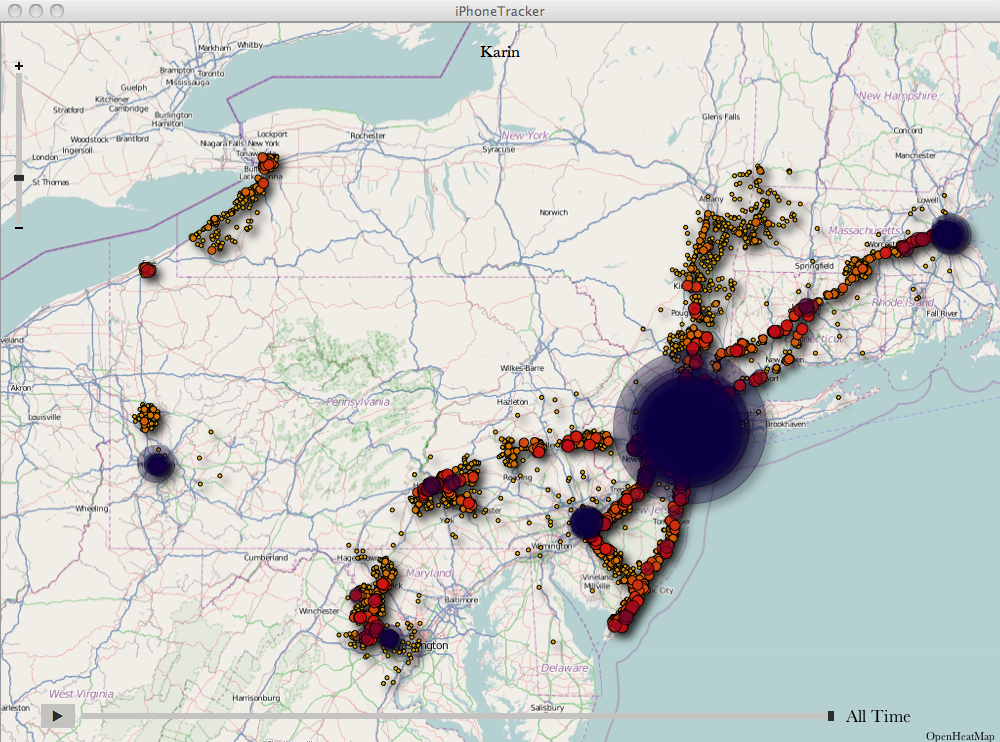
\includegraphics[width=\textwidth]{ch-1/5637893141_ba59f2d989_o.png}
\caption{In April 2011 two researchers discovered that Apple's iOS 4
  operating system recorded the location of nearby Wi-Fi access points
  to aid in geolocation. Due to a bug the database was never
  cleared. As a result, the database could easily be used to create a
  map of every place that the iPhone had been. (C) 2011 John
  Niedermeyer. {\small (Licensed under Creative Commons
  Attribution-NonCommercial-ShareAlike 2.0 Generic)}}.\label{heatmap}
% http://www.flickr.com/photos/nedward/5637893141
\end{figure}


This book is about finding secrets that were present in computer
systems, sent over the Internet or a wireless network, or
inadvertently left in a digital document. 

Over the years a wide variety of programs running on many different
kinds of computers have been responsible for significant privacy and
security violations. The violations are typically
\emph{unintentional}---the people who wrote these programs didn't
create them with the goal of violating privacy. Instead, the programs
have had bugs or usability flaws that caused private information to be
inadvertently retained or distributed. The software problems are
typically so subtle that most users don't realize that their private
information is being compromised. And because the private information
leaked is typically embedded in a form that is invisible or easily
ignored, the flaws can persist for weeks, months, or even years before
they are discovered and fixed.

\section{Technical Privacy Auditing}

This book teaches some of  ways that private information has been
leaked in modern information systems and shows how you can find 
those leaks using tools that are freely available. We call this
process ``technical privacy auditing'' because it uses technical
tools to find privacy problems in software.

Most of the technical privacy failures that we know about were not
discovered by the companies that wrote the software in
question. Instead, they were discovered by students,
journalists, and computer enthusiasts---people who looked at the data
and saw something that they thought was worth investigating.

The root cause of many technical privacy violations is the complexity
of modern information systems. Today's computers are vast, with
gigabytes of storage, tens of thousands of application programs, and
real-time connections to data networks that continually download ever 
more code and data. A typical cell phone with 16 gigabytes of memory can
store literally hundreds of thousands of digital photographs, hours of
video, or months of audio recorded from its internal
microphone. It's very easy for a programmer to overlook some small
piece of storage that may hold some very sensitive piece of
information. 

The basic premise of this book is that many such privacy leaks can be
discovered through straightforward visual inspection---provided that
you know where to look. Our goal is to teach you flexible, general
purpose approaches for finding that data---and provide you with enough
background so that you will understand what you are looking at. This
will put you in the position to discover new privacy and security
leaks in the future.

Privacy leaks such as the hidden information in PDFs and Apple's
unintentional location database are insidious because they are
invisible. They can be present for years in a piece of software that's
used by millions of people. They can be exploited against the interest
of their users. And they are frequently present because nobody looked deeply at the data. 

\subsection{Personally Identifiable Information?}
Most of the leaks described in the previous section share a common
theme: each involved the collection and possible release of personally
identifiable information (PII).

\tk{Explain what PII is}

\subsubsection{Legal definitions}

\tk{Explain legal definition of PII}

\subsubsection{Practical definitions}

\tk{Provide a practical definition of PII}

\subsection{Practical Concerns}


\subsubsection{Reuse of identifiers - at the same time, at different times}
\subsubsection{Shared IDs}
\subsubsection{specificity of identifiers; birthday problem}
\subsubsection{IP addresses}
\subsubsection{Identifiers: IPv4, IPv6, Mobile ID, SIM cards, Phone \#s, email addressses}
\subsection{GUIDs and identifiers}
\subsection{What is ``Unique''}

\section{Digital Forensics Tools}

This book describes how to find leaks of personal information using
digital forensics tools. The previous section gave a brief description
of different kinds of 


The tools that this book introduces for technical privacy auditing are
commonly used for digital forensics and for data
  recovery. \emph{Digital forensics} is a branch of forensic sciences
  that involves the investigation of material found on digital
  devices. Digital Forensics \emph{examiners} employ a variety of
  tools and techniques to find information that might be useful for
  solving a crime, understanding an electronic break-in, or simply
  establishing if information has been stolen or inappropriately
  accessed. 


all too easy for a program to inadvertently collect a piece of private
information and then leave it in memory, save it in a file, or send it
over a network. 

Programs can have privacy-related bugs for years without being noticed 

have been 

Modern computers are extraordinarily complex systems with vast amounts
of storage, high-performance network connections, and all kinds of
sensors. Today a 

Since the dawn of the consumer Internet in the 1990s there have been
many cases in which sensitive information was inadvertently released
because a computer program did not behave properly. 

The secrets are typically
private information that was created and or distributed with a
computer program. 


Over the past 
Typically some user trusted the program to protect
their privacy but it didn't. by a piece
of software that was trusted by their users to protect their privacy
but which failed to do so. We know about 

someone trusted, but that acted in program se secrets were not put
there intentionally---they 

. Specifically, this book is about
finding secrets that are \emph{hidden}, \emph{invisible}, or simply
easy to \emph{overlook}. Secrets that shouldn't be present, but
are. Secrets that are present in computer systems, sent over
information networks, or .

Many 

\section{Detecting data leakage as an experimental science}
\subsection{Detecting data leakage attempts to prove a negative}


Examples in this book should run on Windows, Macintosh and Linux-based
systems. The code was largely developed on a Mac, which is similar to
Linux. 

\section{Conventions used in this book}
In general this book follows \emph{Wikipedia Manual of
  Style}\footnote{\url{http://en.wikipedia.org/wiki/Wikipedia:Manual_of_Style}}
and specifically the Computer
Science\footnote{\url{http://en.wikipedia.org/wiki/Wikipedia:WikiProject_Computer_science/Manual_of_style}}
  and
  Computing\footnote{\url{http://en.wikipedia.org/wiki/Wikipedia:Manual_of_Style/Computing}}
  sections. Specific conventions useful in understanding this book are
  described below.

\subsection{Fonts}

Text in this book is generally typeset in the serif font that you are
now reading. The fixed-width courier font is used for programs,
computer input and output, as well as for numbers that might
reasonably be expected to be constants in a computer program. Thus,
the Earth is 150 million kilometers (150 Gm) from the sun, but a
traditional disk sector has |512| bytes (|512|~B).

\subsection{Radix}
Numbers are generally assumed to be in base 10 unless otherwise
specified. Binary digits will be suffixed with a |b|; octal
is indicated with a leading |0| as in the case in most programming
languages; hexadecimal numbers will have a suffix of an |h| in text
but may be prefixed with |0x| or |\x|. Unfortunately there are
exceptions which must be inferred from context. For example, hex dumps
and cryptographic hashes are always presented courier as unadorned hexadecimal
digits. Examples are shown in \tabref{nomen}.

\begin{table}
\begin{tabular}{rlcrl}
     &              &         & Decimal  \\
Base & Nomenclature & Example & Equivalent      & Usage \\
\hline
2  & Binary      &  |10101111b|& 175            & Text\\
\hline
8  & Octal       &  |0377|     & 255            & Text and code\\
8  & Octal       &  |\377|     & 255            & Code\\
10 & Decimal     &  |1234|     & 1234           & Text and code\\
16 & Hexadecimal &  |DEADBEEFh|& 3,735,928,559  & text \\
   &             &  |0xFF|     & 255            & Output \\
   &             &  |\xFF|     & 255            & Python code\\
\end{tabular}
\caption{Examples of numbers in various bases used in this book.}
\end{table}

\subsubsection{Units}

Natural phenomena discussed in this book are described in Metric
units. Manufactured objects are described in either Metric units or
United States customary units, depending on the system of measurements
that was used to design and produce the object, with approximate
metric units indicated as appropriate. Thus, this book
discusses 5.25-inch (133mm) floppy disks.

\subsection{SI and IEC Multipliers}\label{sec:si-and-iec}
% \note{1MB = 1,000,000 bytes}
% \note{1MiB = 1,048,576 bytes}

Today there are two standards in computing for representing sizes of
files, storage systems, and memory banks: SI (the International System
of Units) decimal prefixes and IEC (International Electrotechnical
Commission) binary prefixes. This situation is confusing because until
recently the SI prefix names \emph{kilo}, \emph{mega} and \emph{giga} were commonly used
for both decimal and binary notation, the correct multiplier being
inferred from usage. Today there is an effort underway to clarify
usage. This section describes correct usage and provides hints for
determining when usage is incorrect.

SI decimal prefixes are commonly used to represent metric
quantities. For example, the SI prefix \emph{giga} multiplies the value that follows by
$10^9$; thus a gigabyte (GB) is
$10^9=1,000,000,000$ bytes. (Confusingly, this is called a billion bytes
in the US but a thousand million bytes in Great Britain, although the
Oxford Dictionary English (British Edition) that ships with MacOS 10.8
calls such usage ``dated.'')

The IEC prefix \emph{gibi} multiples the value following by $2^{30}$. A \emph{gibibyte}
(GiB) is thus $2^{30}=1,073,741,824$ bytes. This has been proper usage
since 1999 when the IEC adopted standard 60027-2 for binary prefixes.

The confusion dates back to the early days of computing, when the ``K''
and ``M'' prefixes were commonly used to mean 1,024 and 1,048,576
when describing memory systems but 1,000 and 1,000,000 when
describing mass storage systems. The difference in terminology resulted
from the way that these systems were addressed. Memory was addressed
by a series of binary address lines, while electromechanical drums and
disks were addressed by specifying a head, a track, and then counting
sector numbers: such numbers only map to even powers-of-two when the
number of heads, tracks and sectors are also even powers-of-two, and
this is rarely the case due to manufacturing concerns.

For much of computing history the correct sense of Ks and Ms could be
inferred from context and, in any event, the difference between 1000
and 1024 wasn't all that significant.

The difference in interpretation became an issue in the 1990s as the
number of people using computers mushroomed and as the commonly used
prefixes went from Ks to Ms and then Gs, resulting in a larger
divergence between the power-of-two measurement and the corresponding
power-of-ten measurement. The IEC prefixes were proposed in
1996\cite{iec:1996},
published as an international standard in 1999, and adopted by the
International Standards organization with the addition of prefixes for
describing exbi (Ei=$2^{60}$), zebi (Zi=$2^{70}$) and yobi (Yi=$2^{80}$) byte
quantities in 2006\cite{iec:80000-13:2008}.  

Despite this standardization effort, today we live in a somewhat
confusing world in which so-called ``4GB'' DRAM modules 
store precisely 4,294,967,296 bytes
but ``4GB'' microSD cards sold for cell
phones store 4,000,000,000 bytes. Even more confusing, the DRAM
module may have four ($2^{2}$) chips, each storing 1073741824
($2^{30}$) bytes each, while the microSD card may two million flash
pages, each with 4096 bytes of usable storage, but present that
information as precisely 7,812,500 logical 512-byte blocks.  These
differences are the result of different operational requirements for
the two kinds of memory, resulting in different kinds of access
electronics, different kinds of software, and different economics. 

It is likely that the IEC binary prefixes will show increased use
with time. Therefore this book uses them to describe block size and
sector size, since they are typically multiples of 512 ($2^9$), but 
SI decimal prefixes are used to describe disk sizes, since that is the way
the devices are sold to consumers.

\section{Other References}
\subsection{Books}\label{section:books}
The following books are referenced in this book:

\printbibliography[heading=bibempty,type=book]


\cite{carrier-file-systems}
\subsection{Articles}
